\chapter{Introduction}
\label{cap:introduction}

This Master's Thesis presents the design and implementation of a complete system for real-time data acquisition, transmission, and visualization inspired by the CanSat concept, whose basic structure is shown in Figure~\ref{fig:cansate}.

The project consists of the construction of a CanSat-type device with different sensors, a Global Navigation Satellite System (GNSS) module, a camera, and communication via Wi-Fi or radio, as well as an open-source web platform in charge of visualizing the collected data in real time.

The platform has been designed as a generic and reusable tool, making it easy to adapt to other similar projects.  
Throughout this document, the context of the work, the motivation, the objectives, the planning, and the overall structure of the thesis are described.

\begin{figure}
    \centering
    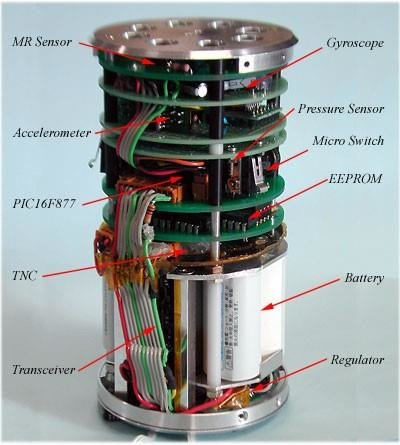
\includegraphics[width=0.5\textwidth]{Imagenes/Bitmap/cansat}
    \caption{Basic diagram of a CanSat. Source: \cite{researchgate_cansat2018}}
    \label{fig:cansate}
\end{figure}

\section{Context}
The CanSat project, whose name comes from the combination of the words \emph{can} and \emph{satellite}, was proposed by Professor Robert J. Twiggs in 1998~\cite{jaxa_cansat}.  
It began as an educational project simulating a nanosatellite with the size of a soda can and a weight of about 350 grams.  
Its objective is to help students of different levels understand all the phases involved in the development of a satellite, from defining the scientific mission to integrating the complete system, including the required sensors, the electronics for operation, the radio transmission to a ground station, the visualization of the data, the design of a 3D-printed enclosure capable of withstanding launch forces, and the design of a parachute.

CanSats are not put into orbit but launched by model rockets, high-altitude balloons, or drones. They are thus subjected to external forces such as acceleration, vibration, or possible impacts, which makes it necessary for them to have a resistant structure.  
The mission of a CanSat is to use its sensors to collect data during descent and transmit them to the ground station.

In recent years, the popularity of CanSats has increased, leading to the creation of national and international competitions promoted by space agencies such as the European Space Agency~\cite{esa_cansat2024}, with the aim of encouraging interest in the aerospace sector and STEM careers in general from an early age.

\section{Motivation}
These projects usually focus on the electronic aspects (data acquisition and transmission), while the visualization of the data often remains underdeveloped.  
In many cases, only basic solutions are implemented, such as console-based visualization or simple plots.  
Moreover, these solutions are often tied to a specific CanSat, which forces each new project to build its visualization solution from scratch.

This highlights the need for a common and reusable platform that allows the real-time visualization of data sent by the CanSat and received by the antenna in a professional and visually clear way, without depending on specific hardware.  
Such a platform would facilitate data analysis during testing and launches and could serve as a base for future project-specific implementations, helping students integrate advanced visualizations without needing to develop a complete platform themselves.

\section{Objectives}
The main objective of this project is to design and develop from scratch a CanSat-type satellite and to implement a reusable data visualization platform.  
The objectives were divided into two main parts: technology research and CanSat development.  
The steps followed in each part are described below.

\begin{itemize}
    \item \textbf{Research}
    \begin{itemize}
        \item Comparison of different microcontrollers and single-board computers to determine which best fit the project objectives.
        \item Study of available sensors on the market and their communication with the microcomputer.
        \item Analysis of different power supply options for the CanSat, including the possibility of using solar panels.
        \item Comparison of current data visualization tools.
    \end{itemize}
    \item \textbf{Development}, divided into two parts: CanSat hardware creation and the visualization platform.
    \begin{itemize}
        \item CanSat
        \begin{itemize}
            \item Construction of a CanSat that complies with the basic size (66 mm × 115 mm) and weight (300–350 g) requirements.
            \item Integration of a GPS receiver.
            \item Camera for real-time video transmission.
            \item Sensors for pressure, temperature, and altitude.
            \item Gyroscope for device orientation.
            \item Battery with solar charging capability.
            \item Data transmission via Wi-Fi when an internet connection is available.
            \item Data transmission via radio when no internet connection is available.
            \item Development of a ground radio receiver.
        \end{itemize}
        \item Visualization platform
        \begin{itemize}
            \item Real-time visualization of all telemetry data received.
            \item Display of the most recent value of each telemetry parameter.
            \item Real-time plots of the received values.
            \item Real-time visualization of transmitted images.
            \item Map with the exact location of the CanSat.
            \item 3D model showing the actual orientation of the CanSat.
            \item Telemetry data download for a selected date range.
        \end{itemize}
    \end{itemize}
\end{itemize}

\section{Work Plan}
The project followed a structured work plan to organize tasks and achieve the proposed objectives.  
This plan was divided into the following steps:

\begin{itemize}
    \item Review and comparison of Arduino and ESP32 microcontrollers and the Raspberry Pi Zero 2 single-board computer, based on their capabilities and compatibility with sensors and communication modules.
    \item Selection of sensors (GNSS, altimeter, and gyroscope), communication module, camera, and power system.
    \item Initial assembly of components on prototyping boards to simplify individual testing.
    \item Definition of the general system architecture, composed of three main components:
    \begin{itemize}
        \item Embedded code in the Raspberry Pi for sensor reading and data transmission.
        \item Ground radio receiver for data sent by the CanSat.
        \item Real-time visualization platform.
    \end{itemize}
    \item Implementation of embedded code on the Raspberry Pi using Python and the appropriate libraries for each sensor.
    \item Implementation of the real-time visualization platform based on events, using RabbitMQ as a message broker, a Java Spring Boot \emph{backend}, a Flutter \emph{frontend}, and a PostgreSQL database to store telemetry data.
    \item Soldering of the components onto a final PCB that complies with the CanSat size requirements.
    \item Integration testing of the complete system, including battery lifetime tests and radio communication range tests.
    \item Writing of the thesis, documenting all steps and results.
\end{itemize}

\section{Source Code and License}
All code developed for this project is available in a single public repository under the MIT license.  
It includes the backend, frontend, and the embedded scripts for both the CanSat and the ground station.  
The repository is hosted on GitHub:

\url{https://github.com/tronxi/real-time-tracking-system}

\section{Thesis Structure}
The thesis is organized into the following chapters:

\begin{itemize}
    \item \textbf{Chapter 1. Introduction:} presents the project context, personal and academic motivation, objectives, and work plan.
    \item \textbf{Chapter 2. Related Work:} reviews previous initiatives related to the CanSat concept, both educational and technical, and analyzes different solutions for data acquisition, transmission, and visualization.
    \item \textbf{Chapter 3. Theoretical Foundations:} defines the technical concepts required for system development, including hardware comparisons, communication technologies, sensors, video protocols, and real-time visualization architectures.
    \item \textbf{Chapter 4. System Design and Implementation:} describes the complete system architecture, the chosen components, the CanSat assembly, the embedded software, the backend, the frontend, and the performed tests.
    \item \textbf{Chapter 5. Conclusions and Future Work:} summarizes the main conclusions of the work, evaluates the results, and proposes possible improvements and future research directions.
\end{itemize}








